\section{Gegen\"uberstellung der Simulations und Messergebnisse}
Ausgehend von den beschriebenen Modellierungsschritten kann nun eine sichere Evaluierung der Kurzschlussanordnungen angesetzt werden. Dabei k\"onnen die Messungen sowie das Simulationsmodell zur Kreuzvalidierung verwendet werden, sodass Mess- und Simulationsfehler weitestgehend auszuschlie\ss{}en sind. Dazu wurde das Simulationsmodell, nach den in Absatz~\ref{ch:sim} versehenen Anpassungen zun\"ach einmal zur Referenz mit den Messungen verglichen. Dazu wird zun\"achst die Testbox ohne Ringkern, jedoch mit fertigem Halterungsaufbau gegen\"ubergestellt. Abbildung~\ref{fig:boxpolycross} zeigt diese Gegen\"uberstellung.
\begin{figure}[htb]
	\centering
	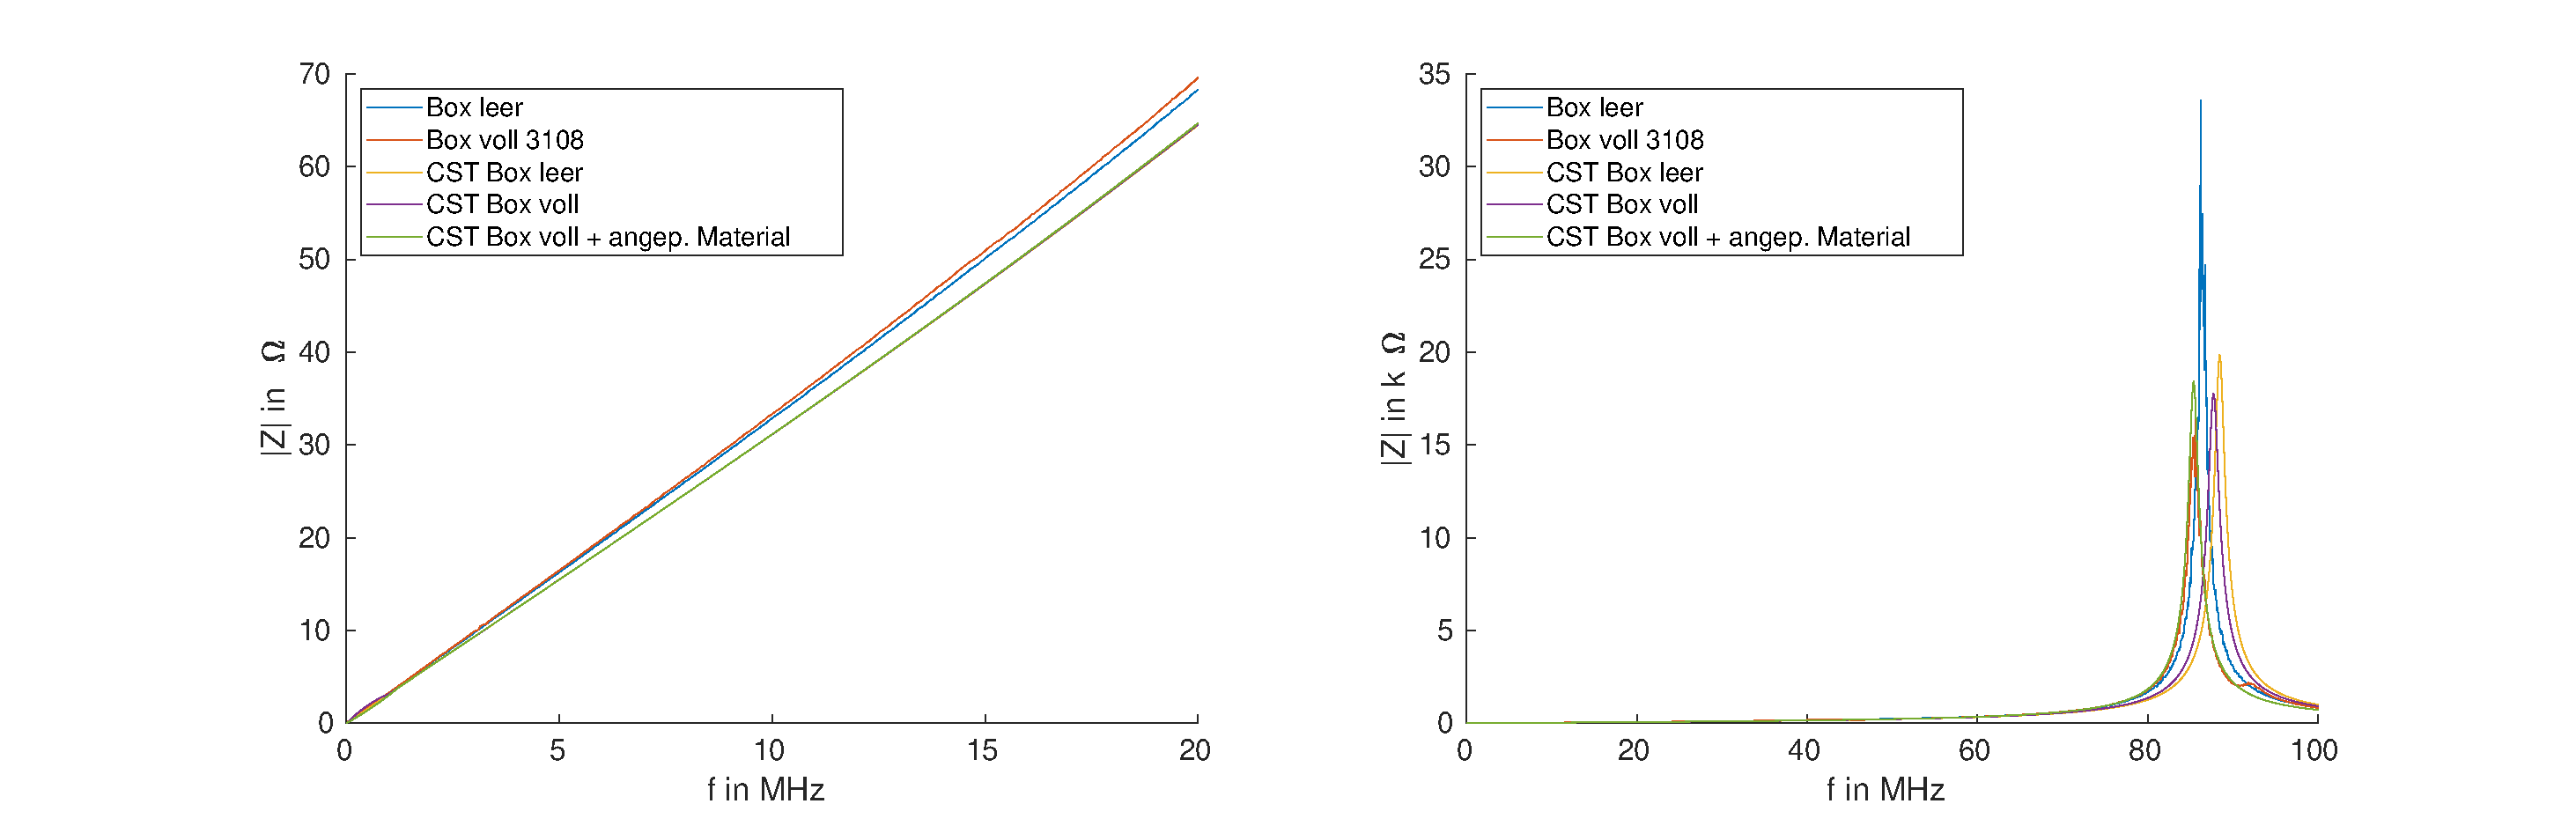
\includegraphics[width=0.95\textwidth]{measurement_simulation_emptybox}
	\caption{Gegen\"uberstellung der Simulation der Box mit Halterung aus Kreuz und Polygon zur entsprechenden Messung.}
	\label{fig:boxpolycross}
\end{figure}
\par
Als n\"achstes in das Modell mit eingesetztem Ringkern zu evalieren. Dazu wird der Ringkern f\"ur die Simulation auf der Position um den Trovidur Ring gelegt, um die reale Box genau abzubilden. Der Aufbau ist in Abbildung~\ref{fig:RKFeRingCST} gezeigt worden. Auch hierbei wird wieder die gemessene Impedanz an der Einkopplung direkt mit der Impedanz aus der Simulation gegen\"ubergestellt. Diese Auswertung ist in Abbildung~\ref{fig:boxpolycrossrk} zu sehen.

\todo[inline,color=red!30]{Plot einf\"ugen}   

\par
Die Gegen\"uberstellung wird f\"ur alle in Abschnitt~\ref{sec:testbox} genannten Kurzschlussanordnungen in gleicher Form durchgef\"uhrt.

\par
Es zeigt sich schnell, dass insbesondere im niedrigen Frequenzbereich eine sehr geringe Abweichung zu erkennen ist. Die Mittlere Abweichung zwischen Simulation und Messung liegt unterhalb von $\SI{20}{\mega\hertz}$ bei nur \todo[inline,color=red!30]{wert und ggf Rechnung einf\"ugen}.   